\chapter{Transformaciones diferenciables}
	\section{Derivadas direccionales}
	
	\begin{defi} Sea $G\subset \R^n$ abierto, sea $a\in G$ y sea $u\in \R^n$ con $\norm{u}=1$. Definimos la \underline{derivada direccional} de $f$ según la dirección del vector $u$ en $a$, como $\limite{\dfrac{f(a+tu)-f(a)}{t}}{t\rightarrow 0}$ siempre que exista dicho límite y lo denotamos como $D_uf(a)$.
	\begin{observacion} Si $\exists D_uf(a)$, entonces $D_uf(a)=\varphi'(0)$ para $\varphi(t)=f(a+tu)$. En efecto:\\ $\varphi'(0)=\limite{}{t\rightarrow0}\ \dfrac{\varphi(t)-\varphi(0)}{t}=\limite{}{t\rightarrow0}\ \dfrac{f(a+tu)-f(a)}{t}=D_uf(a)$.
	\end{observacion}
	\end{defi}
	
	\begin{ejem} Sea $f(x,y)=\sqrt{|x^2+y^2|}\ \forall x,y\in\R^2$\\\\
	¿En qué direcciones $u\ \exists D_uf((0,0))$?\\
	Sea $u\in\R^2$, $\norm{u}=1$, podemos escribir $u=(\cos\theta,\sen\theta)$ con $\theta\in[0,2\pi]$\\ Entonces $\dfrac{f((0,0)+tu)-f(0,0)}{t}=\dfrac{f(0+t\cos\theta,0+t\sen\theta)-f(0,0)}{t}=\\=
	\dfrac{f(t\cos\theta,t\sen\theta)-f(0,0)}{t}=\dfrac{\sqrt{|t^2\cos^2\theta-t^2\sen^2\theta|}-0}{t}=\dfrac{\sqrt{t^2(\cos^2\theta-\sen^2\theta)}}{t}=\\=$
	$\dfrac{|t|\sqrt{\cos^2\theta-\sen^2\theta}}{t}$.\\
	$\doubleleft{\mathrm{Si\ }\sqrt{\cos^2\theta-\sen^2\theta}=0\mathrm{\ entonces \ }\exists\limite{}{t\rightarrow0}\frac{|t|}{t}\sqrt{\cos^2\theta-\sen^2\theta}=0\implies\exists D_{(\cos\theta,\sen\theta)}f(0,0)=0}{\mathrm{Si\ }\sqrt{\cos^2\theta-\sen^2\theta}\neq0\mathrm{\ entonces \ }\nexists\limite{}{t\rightarrow0}\frac{|t|}{t}\sqrt{\cos^2\theta-\sen^2\theta}=0\implies\nexists D_{(\cos\theta,\sen\theta)}f(0,0)=0}$\\
	Lo denotaremos el límite $D_uf(a)$\\
	$\sqrt{\cos^2\theta-\sen^2\theta}=0\iff \cos^2\theta=\sen^2\theta\iff\theta=\left\{\dfrac{\pi}{4},\dfrac{3\pi}{4},\dfrac{5\pi}{4},\dfrac{7\pi}{4}\right\}$\\
	Así $\exists D_uf(0,0)\iff u\in\left\{\left(\dfrac{\sqrt{2}}{2},\dfrac{\sqrt{2}}{2}\right),\left(\dfrac{\sqrt{2}}{2},-\dfrac{\sqrt{2}}{2}\right),\left(-\dfrac{\sqrt{2}}{2},\dfrac{\sqrt{2}}{2}\right),\left(-\dfrac{\sqrt{2}}{2},-\dfrac{\sqrt{2}}{2}\right)\right\}$\\
	¿Qué relación hay entre $D_uf(a)$ y $D_{-u}f(a)$?\\
	Supongamos que $\exists D_uf(a)\iff\limite{}{t\rightarrow0}\dfrac{f(a+tu)-f(a)}{t}$, entonces,\\ ¿existe $\limite{\dfrac{f(a-tu)-f(a)}{t}}{t\rightarrow0}$? Sí, pues $D_{-u}f(a)=\limite{\dfrac{-(f(a-tu)-f(a))}{-t}}{t\rightarrow0}=\\=-\limite{\dfrac{f(a-tu)-f(a)}{-t}}{t\rightarrow0}=-D_uf(a)$.
	\end{ejem}
	
	\section{Derivabilidad y diferenciabilidad}
	\begin{defi} Sea $v\in\R^n\setminus\{0\}$. Se define la derivada de $f$ en $a$ según el vector $v$ como \\ \[\limite{\dfrac{f(a+tv)-f(a)}{t}}{\ttiende}\]
	\begin{nota} No confundir con la derivada direccional de $f$ en $a$ según la dirección de $v$.
	\end{nota}
	\end{defi}
	
	\begin{nota} En $\R^n$ denotamos por $e_i=(0,0,...,\stackbin{\stackbin[\smile]{}{i}}{1},...0)$ para $1\leq i\leq n$ a las derivadas direccionales de $f$ en $a$ según los vectores $e_i$, se les llama derivadas parciales de $f$ en $a$ y se denota por $\dfrac{\partial f}{\partial x_i}(a)$ ó $D_if(a)$.
	\end{nota}
	
	\begin{observacion} Puede ocurrir que $f$ tenga todas las derivadas direccionales en un punto $a$ y no ser continua en $a$.
	\end{observacion}
	
	
	\begin{defi} Si $f$ tiene derivadas parciales en $a$ llamaremos vector gradiente de $f$ en $a$ y lo denotamos $\gradiente f(a)$, al vector $\left(\dfrac{\partial f}{\partial x_1}(a),\dfrac{\partial f}{\partial x_2}(a),...,\dfrac{\partial f}{\partial x_n}(a)\right)$.
	\end{defi}	
	
	\begin{ejem} Sea $f(x,y)=3x^2+y^3$ el vector gradiente de $f$ en un punto $(x,y)\in\R^2$ es $\gradiente f(x,y)=\left(\dfrac{\partial f}{\partial x}(x,y),\dfrac{\partial f}{\partial y}(x,y)\right)=(6x,3y^2)$.
	\end{ejem}
	
	\begin{observacion} Sea $D\subset\R$, si $\function{f}{D}{\R}$ es derivable en $a$, se tiene:\\
	$f'(a)=\limite{\dfrac{f(a+h)-f(a)}{h}}{\htiende}=\limite{\dfrac{f(x)-f(a)}{x-a}}{x\rightarrow a}\implies 0=\limite{\left(\dfrac{f(a+h)-f(a)}{h}-f'(a)\right)}{\htiende}=\\=\limite{\left(\dfrac{f(a+h)-f(a)-f'(a)h}{h}\right)}{\htiende}$ y observamos que la aplicación $h\longrightarrow f'(a)h$ es una aplicación lineal de $\R$ en $\R\iff\limite{\dfrac{f(a+h)-f(a)-f'(a)h}{|h|}}{\htiende}=0$ 
	\end{observacion}
	
	\begin{defi} Sea $U\subset\R^n$ abierto, sea $\function{f}{U}{\R}$ y sea $a\in U$, diremos que $f$ es \underline{diferenciable} en $a$ si existe una aplicación lineal $L\colon\R^n\longrightarrow\R$ tal que:\\ \\
	$\limite{\dfrac{f(a+h)-f(a)-L(h)}{\norm{h}}}{\htiende}=0\iff\limite{\dfrac{|f(a+h)-f(a)-L(h)|}{\norm{h}}}{\htiende}=0\iff\\\iff\limite{\dfrac{f(x)-f(a)-L(x-a)}{\norm{x-a}}}{x\to a}=0$
	\begin{nota} Si existe tal aplicación lineal $L$, entonces es única. Será consecuencia de la siguiente proposición.
	\end{nota}
	\end{defi}
	
	\begin{proposicion} Sea $U\subset\R^n$ abierto, sea $\function{f}{U}{\R}$ y sea $a\in U$. Si $f$ es diferenciable en $a$, entonces existen todas las derivadas direccionales de $f$ en $a$. Además, si $L$ es una aplicación lineal que cumple $\limite{\dfrac{f(a+h)-f(a)-L(h)}{\norm{h}}}{\htiende}=0$, se tiene que $D_uf(a)=L(u)\ \forall u\in\R^n$ con $\norm{u}=1$.
	\begin{proof}\ \\
	Por hipótesis $\exists L\colon \R^n\longrightarrow\R$ lineal tal que $\limite{\dfrac{f(a+h)-f(a)-L(h)}{\norm{h}}}{\htiende}=0$.\\
	Sea $u\in\R^n$ y $||u||=1$. Por lo anterior $\limite{\dfrac{f(a+tu)-f(a)-L(tu)}{\norm{tu}}}{\ttiende}=\\=\stackbin[h=tu]{}{\limite{}{\htiende}}\dfrac{f(a+h)-f(a)-L(h)}{\norm{h}}\implies\limite{\dfrac{f(a+tu)-f(a)-tL(u)}{|t|}}{\ttiende}=0\implies$\\
	$\implies \limite{\dfrac{f(a+tu)-f(a)-tL(u)}{t}}{\ttiende}=0\implies\limite{\dfrac{f(a+tu)-f(a)}{t}-L(u)}{\ttiende}=0\implies\\\implies
	\exists \limite{\dfrac{f(a+tu)-f(a)}{t}=L(u)}{\ttiende}\iff\exists D_uf(a)=L(u)$
	\end{proof}
	\end{proposicion}
	
	\begin{corolario}$L(a_i)=\dfrac{\partial f}{\partial x_i}(a)$, para $1\leq i\leq n$, como $L$ es lineal, está unívocamente determinado por sus valores en los vectores en la base cánonica de $\R^n$.\\ Así que si $f$ es diferenciable en $a$, la aplicación lineal $L\colon \R^n\to\R$ es la que tiene por matriz asociada $\left(\dfrac{\partial f}{\partial x_1}(a),\dfrac{\partial f}{\partial x_2}(a),...,\dfrac{\partial f}{\partial x_n}(a) \right)$ y $L(h)=\dfrac{\partial f}{\partial x_1}(a)h_1+\dfrac{\partial f}{\partial x_2}(a)h_2+...+\dfrac{\partial f}{\partial x_n}(a)h_n=\\=
	\dotproduct{\gradiente f(a)}{h}$\\\\
	Si $f$ es diferenciable en $a$ a la aplicación $L$ anterior le llamamos diferencial de $f$ en $a$ y la denotamos $df(a)$. Por tanto $df(a)\colon\R^n\to\R$ es lineal y se tiene que $df(a)(h)=\dotproduct{\gradiente f(a)}{h}\ \forall h\in\R^n$
	\end{corolario}
	
	\begin{proposicion} Sea $U\subset\R^n$ abierto, sea $\function{f}{U}{\R}$ y sea $a\in U$. Si $f$ es diferenciable en $a\implies f$ es continua en $a$.
	\begin{proof}\ \\
	Por hipótesis $\limite{\dfrac{f(a+h)-f(a)-\dotproduct{\gradiente f(a)}{h}}{\norm{h}}}{\htiende}=0$\\ Para $\varepsilon_0=1\ \exists r>0\talque$ si $h\in B(\overline{0},r)\setminus\{\overline{0}\}$ se tiene $\dfrac{f(a+h)-f(a)-\dotproduct{\gradiente f(a)}{h}}{\norm{h}}<1$\\
	Queremos probar que $f$ es continua en $a$; es decir, que $\limite{f(x)}{x\to a}=f(a)\iff\limite{f(a+h)-f(a)}{\htiende}=0\iff \limite{}{\htiende}\norm{f(a+h)-f(a)}=0$\\
	$\forall x\in B(a,r)\setminus\{a\}$ tenemos $0\leq |f(x)-f(a)|=\\=\norm{x-a}\left|\dfrac{f(x)-f(a)-\dotproduct{\gradiente f(a)}{x-a}}{\norm{x-a}}+\dfrac{\dotproduct{\gradiente f(a)}{x-a}}{\norm{x-a}}\right|\leq\\\leq\norm{x-a}\left|\left(\dfrac{f(x)-f(a)-\dotproduct{\gradiente f(a)}{x-a}}{\norm{x-a}}\right)\right|+\left|\dotproduct{\gradiente f(a)}{x-a}\right|\leq\\\stackbin[\mathrm{por\ Cauchy-Schwarz}]{\mathrm{por\ }0\leq\norm{x-a}\leq r}\leq\norm{x-a}+\norm{\gradiente f(a)}\norm{x-a}=\norm{x-a}(1+\norm{\gradiente f(a)})$\\\\
	Es decir, $\ 0\leq|f(x)-f(a)|\leq\norm{x-a}(1+\norm{\gradiente f(a)})\ \forall x\in B(a,r)\setminus\{a\}$.\\
	Como $\limite{\norm{x-a}(1+\norm{\gradiente f(a)})}{x\to a}=0$, por el criterio de  compresión deducimos que\\ $\limite{(f(x)-f(a))}{x\to a}=0.\ $ Esto es $\limite{f(x)}{x\to a}=f(a)\implies f$ continua en $a$.
	\end{proof}
	\end{proposicion}
	
	\begin{observacion} Existen funciones con todas las derivadas direccionales en un punto $a$ y no son diferenciables en $a$.
	\end{observacion}
	
	\begin{lema}\underline{Importante}. Si $f$ es diferenciable en $a$, entonces:\\\\
	$\limite{\dfrac{f(a+h)-f(a)-df(a)(h)}{\norm{h}}}{\htiende}=0\iff\limite{\dfrac{f(a+h)-(f(a)+df(a)(h))}{\norm{h}}}{\htiende}=0$\\
	Esto es que ``cerca de 0'' tenemos que $f(a+h)$ es ``aproximadamente'' $f(a)+df(a)(h)$; o equivalentemente, ``cerca de $a$'', el valor de $f(x)$ es ``aproximadamente'' $f(a)+df(a)(x-a)$.\\\\
	A la gráfica de la función $g(x)\colon=f(a)+df(a)(x-a)$, le llamamos recta, plano o hiperplano (según la dimensión de $\R^n$) tangente en la gráfica de $f$ en el punto $(a,f(a))$.\\
	Esto es el plano tangente a la gráfica de $f$ en $(a,f(a))$ correspondiente con el conjunto\\ $T:=\left\{x=(x_1,x_2,...,x_n,x_{n+1})\in \R^{n+1}\talque x_{n+1}=f(a_1,a_2,...,a_n)+\stackbin[i=1]{n}\sum\dfrac{\partial f}{\partial x_i}(a)(x_i-a_i)\right\}$\\\\
	En la siguiente gráfica de la función $f(x)=x^2$, tenemos la recta tangente al punto $a=1$
	\begin{figura}\ \\
	\begin{tikzpicture}
	\begin{axis}[axis lines = left, xlabel =$x$, ylabel=$f(x)$,xmin=0,xmax=5,ymin=0,ymax=5]
		\addplot[samples = 100, color = red]{x^2};\addlegendentry{$f(x)=x^2$}
		\addplot[domain=0:5]{2*x-1};
		\addplot coordinates{(1,1)};
	\end{axis}
	\end{tikzpicture}
	\end{figura}
	\end{lema}
	
	\begin{ejem} Probar que $f(x,y)=x^2+y^3-2x-y+5$ es diferenciable en $(0,0)$ y hallar el plano tangente a dicho punto.\\
	$\tripleright{\dfrac{\partial f}{\partial x}(x,y)=2x-2}{}{\dfrac{\partial f}{\partial y}(x,y)=3y^2-1}\implies\triple{\dfrac{\partial f}{\partial x}(0,0)=-2}{}{\dfrac{\partial f}{\partial y}(0,0)=-1}$\\
	¿$f$ es diferenciable en $(0,0)$?$\iff$¿$\exists\limite{\dfrac{f(x,y)-f(0,0)-\dotproduct{\gradiente f(0,0)}{(x-0,y-0)}}{\norm{(x-0,y-0)}}}{(x,y)\to (0,0)}=\\=0\iff \limite{\dfrac{f(x,y)-f(0,0)-(-2x+(-y))}{\norm{(x,y)}}}{(x,y)\to (0,0)}=0$ ?\\\\
	Entonces, $0\leq \dfrac{|f(x,y)-f(0,0)+2x+y|}{\sqrt{x^2+y^2}}=\dfrac{|x^2+y^3-2x-y+5-5+2x+y|}{\sqrt{x^2+y^2}}=\dfrac{|x^2+y^3|}{\sqrt{x^2+y^2}}\leq\\\leq\dfrac{x^2}{\sqrt{x^2+y^2}}+\dfrac{|y|y^2}{\sqrt{x^2+y^2}}=|x|\sqrt{\dfrac{|x|^2}{x^2+y^2}}+y^2\sqrt{\dfrac{|y|^2}{x^2+y^2}}\leq|x|+|y|^2\ \forall(x,y)\in \R^2\setminus\{(0,0)\}$\\\\
	Como $\limite{|x|+|y|^2}{(x,y)\to (0,0)}=0$, por el criterio de compresión, $\\\limite{\dfrac{f(x,y)-f(0,0)-(-2x+(-y))}{\sqrt{x^2+y^2}}}{(x,y)\to (0,0)}=0\ $ luego $f$ es diferenciable en $(0,0)$ y \\
	$df(0,0)\colon \stackbin[(h,k)\to-2h- k]{}{\R^2\to\R}$\\
	Entonces $df(0,0)(h,k)=-2h-k\ \forall h,k\in\R^2$. El plano tangente en la gráfica de $f$ en $(0,0,5)=(0,0,f(0,0))$ tiene por ecuación:\\
	$\tau=f(0,0)+df(0,0)((x-0),(y-0))=5+df(0,0)(x,y)=5-2x-y$
	\begin{figura}\ \\
	\begin{center}
	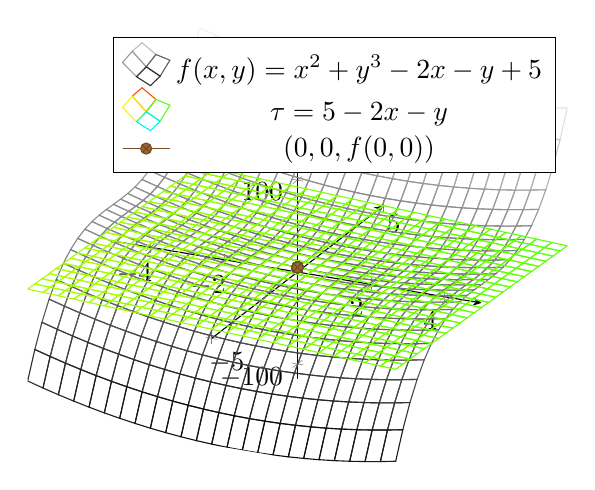
\begin{tikzpicture}
	\begin{axis} [axis lines=middle]
	\addplot3[mesh,colormap/blackwhite]{x^2+y^3-2*x-y+5};\addlegendentry{$f(x,y)=x^2+y^3-2x-y+5$}
	\addplot3[mesh,colormap/bluered]{5-2*x-y};\addlegendentry{$\tau=5-2x-y$}
	\addplot3 ({0},{0},{5});\addlegendentry{$(0,0,f(0,0))$}
	\end{axis}
	\end{tikzpicture}
	\end{center}
	\end{figura}
	\end{ejem}
	
	\begin{observacion} Como consecuencia del ejercicio anterior:\\
	$f(x)=f(a)+df(a)(x-a)+\varphi(x)$ donde $\varphi$ cumple $\limite{\dfrac{f(x)}{\norm{x-a}}}{x\to a}=0$
	\end{observacion}
	
	\begin{ejem} Aproximar $(0,99\cdot \e^{0,02})^{8}$\\
	Consideramos la función $f(x,y)=(x\e^y)^8=x^8\e^{8y}$. Calculemos $f(0'99,0'02)$\\
	$(0,99\cdot \e^{0,02})^{8}=f(0'99,0'02)\approx f(1,0)+df(1,0)(0'99-1,0'02-0)=\\=1+\dotproduct{\gradiente f(1,0)}{(-0'01,0'02)}=1+\dotproduct{(8,8)}{(-0'01,0'02)}=1+8(-0'01+0'02)=1,08$
	\end{ejem}
	
	\begin{proposicion} Condición suficiente de diferenciabilidad.\\
	Sea $U\in\R^n$ abierto, sea $\function{f}{U}{\R}$ y sea $a\in U$. Si $\exists r>0\talque$ en $B(a,r)$ existen las derivadas parciales de $f$ y son continuas en $a$, entonces $f$ es diferenciable en $a$.
	\begin{proof}\ \\
	Queremos probar que $\limite{\dfrac{f(x)-f(a)-\stackbin[i=1]{n}\sum \dfrac{\partial f}{\partial x_i}(a)(x_i-a_i)}{\norm{x-a}}}{x\to a}=0$\\
	Sea $x\in B(a,r)\setminus\{a\}$, entonces, $f(x_1,x_2,...,x_n)-f(a_1,a_2,...,a_n)=\\=
	f(x_1,x_2,...,x_n)-f(a_1,x_2,...,x_n)+f(a_1,x_2,...,x_n)-f(a_1,a_2,x_3,...,x_n)+f(a_1,a_2,x_3,...,x_n)+\\+...-f(a_1,a_2,...,a_{n-1},x_n)+f(a_1,a_2,...,a_{n-1},x_n)-f(a_1,a_2,...,a_n)$\\
	Para cada $i\in\{1,2,...,n\}$ podemos aplicar el teorema del valor medio a la función $\varphi_i(t)=\\=f(a_1,a_2,...,t_i,x_{i+1},...,x_n)$ y obtenemos que $\exists t_i$ entre $x_i$ y $a_i$ tal que $\varphi_i'(t_i)=\dfrac{\varphi(x_i)-\varphi(a_i)}{x_i-a_i}\implies\\ \implies \varphi(x_i)-\varphi(a_i)=\varphi_i'(t_i)(x_i-a_i)=\dfrac{\partial f}{\partial x_i}(a_1,a_2,...,t_i,x_{i+1},...,x_n)(x_i-a_i)$\\
	Por tanto, sea $U_i=(a_1,a_2,...,t_i,x_{i+1},...,x_n)$ tenemos que $\norm{U_i-a}\leq\norm{x-a}$\\
	$f(x)-f(a)=\stackbin[i=1]{n}\sum(\varphi_i(x_i)-\varphi_i(a_i))\stackbin{\mathrm{TVM}}=\stackbin[i=1]{n}\sum\dfrac{\partial f}{\partial x_i} (U_i)(x_i-a_i)$, veamos que tiende a 0.\\
	Por tanto: $0\leq \dfrac{1}{\norm{x-a}}\left|f(x)-f(a)-\stackbin[i=1]{n}\sum\dfrac{\partial f}{\partial x_i}(a)(x_i-a_i)\right|=\\=\dfrac{1}{\norm{x-a}}\left|\stackbin[i=1]{n}\sum\dfrac{\partial f}{\partial x_i} (U_i)(x_i-a_i)-\stackbin[i=1]{n}\sum\dfrac{\partial f}{\partial x_i}(a)(x_i-a_i)\right|\leq\\ \leq \dfrac{1}{\norm{x-a}}\stackbin[i=1]{n}\sum\left|\dfrac{\partial f}{\partial x_i}(U_i)-\dfrac{\partial f}{\partial x_i}(a)\right||x_i-a_i|\leq\dfrac{1}{\norm{x-a}}\cdot\norm{x-a}\stackbin[i=1]{n}\sum\left|\dfrac{\partial f}{\partial x_i}(U_i)-\dfrac{\partial f}{\partial x_i}(a)\right|=\\=
	\stackbin[i=1]{n}\sum\left|\dfrac{\partial f}{\partial x_i}(U_i)-\dfrac{\partial f}{\partial x_i}(a)\right|$\\
	Así, dado $\varepsilon>0$, $\dfrac{\partial f}{\partial x_i}$ es continua en $a$ $\forall i\in\{1,2,...,n\}$, entonces $\exists \delta_1,\delta_2,...,\delta_n>0$ tal que:\\
	$\left|\dfrac{\partial f}{\partial x_i}(x)-\dfrac{f}{x_i}(a)\right|<\dfrac{\varepsilon}{n}\ \forall x\in B(a,\delta_i)$. Tomemos $\delta = \min\{\delta_1,...,\delta_n\}>0$.\\
	Ahora, si $x\in B(a,\delta)\setminus\{a\}$ tenemos que:\\
	$0\leq\dfrac{1}{\norm{x-a}}\left|f(x)-f(a)-\stackbin[i=1]{n}\sum\dfrac{\partial f}{\partial x_i}(a)(x_i-a_i)\right|\leq 
	\stackbin[i=1]{n}\sum\left|\dfrac{\partial f}{\partial x_i}(U_i)-\dfrac{\partial f}{\partial x_i}(a)\right|\leq\stackbin[i=1]{n}\sum\dfrac{\varepsilon}{n}=\varepsilon$
	\end{proof}
	\end{proposicion}
	
	\begin{observacion}Como consecuencia de la proposición anterior, si $\function{f}{U}{\R}$ tiene derivadas parciales y son continuas en $U\subset\R^n$ abierto, entonces $f$ es diferenciable en $u\ \forall u\in U$.
	\end{observacion}
	
	\begin{ejem} Estudia la diferenciabilidad de:\\
	$f(x,y)=\doubleleft{\dfrac{xy^2}{x^2+y^4}\mathrm{\ si\ }(x,y)\neq(0,0)}{\ \ \ \ 0\mathrm{\ \ \ \ \ \ si\ }(x,y)=(0,0)}$\\
	Es claro que $g(x)=\dfrac{xy^2}{x^2+y^4}$ tiene derivadas parciales y son continuas en todo su dominio, $D_g=\R^2\setminus\{(0,0)\}$ y $f\equiv g$ en $\R^2\setminus\{(0,0)\}$. Entonces $f$ tiene derivadas parciales y son continuas en $\R^2\setminus\{(0,0)\}$\\
	Por la proposición anterior, tenemos que $f$ es diferenciable en $\R^2\setminus\{(0,0)\}$. Veamos que ocurre en $(0,0)$. Podemos comprobar que $f$ tiene todas las derivadas direccionales en $(0,0)$, pero $f$ no es diferenciable en $(0,0)$ entre otras cosas porque no es continua en dicho punto.\\ De hecho $\nexists \limite{f(x,y)}{(x,y)\to(0,0)}$. En efecto:\\
	$\limite{f(x,0)}{x\to 0}=0$\\
	$\limite{f(x^2,x)}{x\to 0}=\limite{\dfrac{x^2x^2}{x^4+x^4}}{x\to 0}=\limite{\dfrac{x^4}{2x^4}}{x\to 0}=\dfrac{1}{2}\neq 0$
	\begin{figura}\ \\
	\begin{center}
	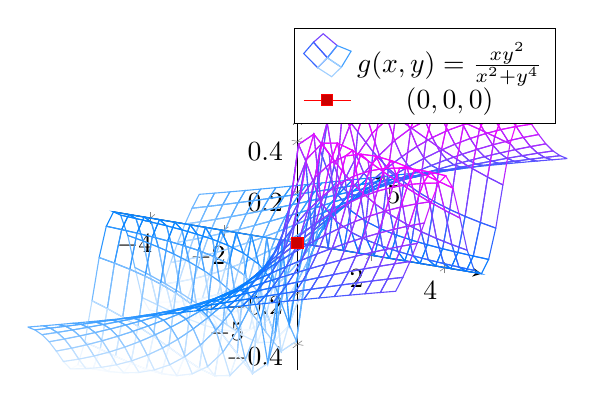
\begin{tikzpicture}
	\begin{axis} [axis lines=middle]
	\addplot3[mesh,colormap/cool, domain=-5:5]{(x*y^2)/(x^2+y^4)};\addlegendentry{$g(x,y)=\frac{xy^2}{x^2+y^4}$}
	\addplot3 ({0},{0},{0}); \addlegendentry{$(0,0,0)$}
	\end{axis}
	\end{tikzpicture}
	\end{center}
	\end{figura}
	\end{ejem}
	
	\begin{observacion}\ \\
	Sea $\doubleright{g\mathrm{\ diferenciable\ en \ }B}{f\equiv g\mathrm{\ en \ }B}\implies f$ es diferenciable en $\mathring{B}$ y $df(a)=dg(a)\ \forall a\in\mathring{B}$
	\end{observacion}
	
	\begin{observacion} Si $f$ es diferenciable en $a$, entonces $f$ es continua en $a$ y tiene todas las derivadas parciales de $f$ en $a$. Además $D_uf(a)=\dotproduct{\gradiente f(a)}{u}\ \forall u\in\R^n$ con $\norm{u}=1$\\
	Como $\dotproduct{\gradiente f(a)}{u}=\norm{\gradiente f(a)} \  \norm{u}\cos(\gradiente f(a),u)=\norm{\gradiente f(a)}\cos(\gradiente f(a),u)$.\\
	Por tanto la derivada direccional maximal de $f$ en $a$ se alcanza en la dirección del vector gradiente $\gradiente f(a)=\left(\dfrac{\partial f}{\partial x_1}(a),\dfrac{\partial f}{\partial x_2}(a),...,\dfrac{\partial f}{\partial x_n}(a)\right)$ y su valor es $\norm{\gradiente f(a)}$.
	\end{observacion}
	
	\section{Diferenciabilidad en funciones de $\R^n$ en $\R^m$}	
	
	\begin{nota} Antes de continuar conviene leer el Apéndice \textsc{A. Repaso de aplicaciones lineales}.\end{nota}
	
	\begin{defi} Sea $U\in \R^n$ abierto, $\xfunction{f}{U}{\R^m}{x\rightarrow(f_1(x),f_2(x),...,f_m(x))}$ y sea $a\in U$. Diremos que $f$ es \textbf{diferenciable en $a$} si $\exists \function{L}{\R^n}{\R^m}$ lineal tal que $\limite{\dfrac{f(a+h)-f(a)-L(h)}{\norm{h}}}{\htiende}=\overline{0}\in\R^m$ o equivalentemente, $\limite{\dfrac{f(x)-f(a)-L(x-a)}{\norm{x-a}}}{x\rightarrow a}=\overline{0}\iff \limite{\dfrac{\norm{f(x)-f(a)-L(x-a)}_{\R^m}}{\norm{x-a}_{\R^n}}}{x\rightarrow a}=\\=0$.
	\begin{observacion} $\limite{\dfrac{f(a+h)-f(a)-L(h)}{\norm{h}}}{\htiende}=\overline{0}\in\R^m\iff \limite{\dfrac{f_i(a+h)-f_i(a)-L_i(h)}{\norm{h}}}{\htiende}=\\=0\in\R$, para $1\leq i\leq m\iff L_i=df_i(a)$ para $1\leq i\leq m$.
	\end{observacion}
	Veamos ahora que si existe dicha $L$, ha de ser $L=(L_,L_2,...,L_m)=(df_1(a),df_2(a),...,df_m(a))$.\\
	Por tanto si existe $L$, es única, la llamamos diferencial de $f$ en $a$ y la denotamos por $df(a)$.
	\begin{observacion}
	$f=(f_1,f_2,f_3,..,f_m)$ es diferenciable en $a\iff f_1,f_2,..,f_m$ son diferenciables en $a$. Además $df(a)=(df_1(a),df_2(a),...,df_m(a))$\\
	Así tenemos que $f$ diferenciable en $a\implies f$ continua en $a$ ya que, $f$ diferenciable en $a\implies f_1,f_2,...,f_m$ diferenciables en $a\implies f_1,f_2,...,f_m$ continuas en $a\implies f$ es continua en $a$.\\
	\end{observacion}
	\end{defi}
	
	\begin{defi} A la matriz asociada a $df(a)$ la denominamos \textbf{matriz jacobiana de $f$ en $a$} y la denotamos por $J_f(a)$.\\
	$J_f(a)=\begin{pmatrix}
	\dfrac{\partial f_1}{\partial x_1}(a) & \dfrac{\partial f_1}{\partial x_2}(a) & \ldots & \dfrac{\partial f_1}{\partial x_n}(a)\\ \dfrac{\partial f_2}{\partial x_1}(a)& \ddots & &\vdots\\ \vdots & & \ddots & \vdots\\ \dfrac{\partial f_m}{\partial x_1}(a)& \ldots & \ldots & \dfrac{\partial f_m}{\partial x_n}(a)
	\end{pmatrix}=\begin{pmatrix}
	D_1f_1(a) & D_2f_1(a) & \ldots & D_nf_1(a)\\ D_1f_2(a)& \ddots & &\vdots\\ \vdots & & \ddots & \vdots\\ D_1f_m(a)& \ldots & \ldots & D_mf_n(a)
	\end{pmatrix}$
	\end{defi}
	
	\begin{ejem} $\xfunction{f}{\R^3}{\R^2}{(x,y,z)\rightarrow(x^2y,3zy^3)}$\\
	$f$ es diferenciable en todo $\R^3$ pues $f_1(x,y,z)=x^2y$ y $f_2(x,y,z)=3zy^3$ tienen derivadas parciales y son continuas en $\R^3$ luego son diferenciables en $\R^3$\\
	$J_f(x,y,z)=\begin{pmatrix} 2xy&x^2&0\\0&9zy^2&3y^3	
	\end{pmatrix}$ en particular $J_f(1,0,2)=\begin{pmatrix}0&1&0\\0&0&0\end{pmatrix}$\\
	$\function{df(1,0,2)}{\R^3}{\R^2}$ donde $(h_1,h_2,h_3)\rightarrow \begin{pmatrix}
	J_f(1,0,2)\begin{pmatrix}h_1\\h_2\\h_3	\end{pmatrix}\end{pmatrix}^t=\begin{pmatrix}
	\begin{pmatrix}0&1&0\\0&0&0	\end{pmatrix} &\begin{pmatrix}h_1\\h_2\\h_3\\	\end{pmatrix}
	\end{pmatrix}^t=\\=\begin{pmatrix}h_2\\0	\end{pmatrix}^t=\begin{pmatrix}h_2 & 0	\end{pmatrix}. $
	\end{ejem}
	
	\begin{ejem} $\xfunction{f}{\R}{\R^3}{t\to (\cos t,\sen t, t)}$\\
	$f_1,f_2,f_3$ son continuas en $\R$, luego $f$ es diferenciable en $\R$ y tenemos:\\
	$J_f(t)=\begin{pmatrix}f_1'(t)\\f_2'(t)\\f_3'(t)\end{pmatrix}= \begin{pmatrix}-\sen(t)\\\cos(t)\\1\end{pmatrix}$
	\end{ejem}
	
	\section{Propiedades de la diferenciabilidad de funciones de $\R^n$ en $\R^m$}	
	
	\begin{proposicion} Sea $U\subset \R^n$ abierto, sean $\function{f\mathrm{\ y\ }g}{U}{\R^m}$ y sea $a\in U$. Si $f$ y $g$ son diferenciables en $a$ entonces $(f+g)$, $(f-g)$ y $\alpha f$ (con $\alpha \in \R$) son diferenciables en $a$ y además:\begin{itemize}
	\item $d(f+g)(a)=df(a)+dg(a)$
	\item $d(f-g)(a)=df(a)-dg(a)$
	\item $d(\alpha f)(a)=\alpha df(a)$
	\end{itemize}
	\begin{proof}\ \\
	A partir de la definición de diferenciabilidad y de la proposición de los límites.	
	\end{proof}
	\end{proposicion}
	
	\begin{teor}\textbf{Regla de la cadena}.\\
		Sea $U\subset \R^n$ abierto, sea $V\subset\R^m$ abierto, sea $\function{f}{U}{\R^m}$, sea $\function{g}{V}{\R^k}$ tal que $f(U)\subset V$ y sea $a\in U$. Si $f$ es diferenciable en $a$ y $g$ es diferenciable en $f(a)$, entonces $g\circ f$ es diferenciable en $a$ y $d(g\circ f)(a)=dg(f(a))\circ df(a)$ y por tanto $J_{g\circ f}(a)=J_g(f(a))\cdot J_f(a)$.
		\begin{ejem} Sean $f(x,y,z)=(x^2y,y+z)$ y $g(u,v)=u\cdot v$ $(\R^3\overset{f}\to\R^2\overset{g}\to \R)$ \\
			$J_{g\circ f}(x,y,z)=J_g(f(x,y,z))\cdot J_f(x,y,z)$
		\end{ejem}
		\begin{proof}\ \\
		Por hipótesis, sea $L=df(a)$ y $S=dg(f(a))$, tenemos:\\
		\begin{enumerate}[a)]
			\item $\dfrac{f(x)-f(a)-L(x-a)}{\norm{x-a}}\overset{x\to a}\longrightarrow 0\ (\in\R^m)$
			\item $\dfrac{g(y)-g(f(a))-S(y-f(a))}{\norm{y-f(a)}}\overset{y\to f(a)}\longrightarrow 0\ (\in\R^k)$
		\end{enumerate}
		Queremos probar:
		\[\dfrac{g(f(x))-g(f(a))-S\circ L(x-a)}{\norm{x-a}}\overset{x\to a}\longrightarrow 0\ (\in\R^k)\]
		Entonces:\\
		Por a), para $\varepsilon_0=1\ \exists r>0 \talque \dfrac{\norm{f(x)-f(a)-L(x-a)}}{\norm{x-a}} < 1\ \forall x\in B(a,r)\setminus\{a\}\implies$\\
		$\implies\norm{f(x)-f(a)-L(x-a)}\leq \norm{x-a}\ \forall x\in B(a,r)\implies \norm{f(x)-f(a)}\leq\\\leq\norm{f(x)-f(a)-L(x-a)}+\norm{L(x-a)}\leq\norm{x-a}+\norm{L}\norm{x-a}=(1+\norm{L})\norm{x-a}\ \forall x\in B(a,r)$\\
		Así tenemos $f$ diferenciable en $a\implies\exists r>0\ \exists M>0 \talque \norm{f(x)-f(a)}\leq M\norm{x-a}\ \forall x\in B(a,r)$\\
		Dado $\varepsilon >0$, buscamos $\delta >0 \talque \dfrac{\norm{g(f(x))-g(f(a))-S\circ L(x-a)}}{\norm{x-a}}<\varepsilon\ \forall x\in B(a,\delta)\setminus\{a\}$\\
		Para $\varepsilon' = \dfrac{\varepsilon}{2(\norm{S}+1)}>0$, por a), tenemos que $\exists\delta_1>0$ tal que:\\
		$\boxed{\dfrac{\norm{f(x)-f(a)-L(x-a)}}{\norm{x-a}}<\varepsilon'\ \forall x \in B(a,\delta_1)\setminus\{a\}}^{\textbf{(*)}}$\\
		Para $\varepsilon'' = \dfrac{\varepsilon}{2M}>0\ \exists\delta_2>0 \talque \dfrac{\norm{g(y)-g(f(a))-S(y-f(a))}}{\norm{y-f(a)}}<\varepsilon''\ \forall y \in B(f(a),\delta_2)\setminus\{f(a)\}\\
		\implies\boxed{\norm{g(y)-g(f(a))-S(y-f(a))}<\varepsilon''\norm{y-f(a)}\ \forall y\in B(f(a),\delta_2)}^{\textbf{(**)}}$\\
		Sea $\delta=\min\{r,\delta_1,\delta_2\}>0$. Ahora si $x\in B(a,\delta)\setminus\{a\}$; es decir, $0<\norm{x-a}<\delta$ tenemos:\\
		$\dfrac{\norm{g(f(x))-g(f(a))-S\circ L(x-a)}}{\norm{x-a}}\stackbin[+\mathrm{\ des.\ triangular}]{\pm S(f(x)-f(a))}\leq\dfrac{\norm{g(f(x))-g(f(a))-S(f(x)-f(a))}}{\norm{x-a}} +\\+ \dfrac{\norm{S(f(x)-f((a))-S\circ L(x-a)}}{\norm{x-a}}$ y ahora por (**) y como $\norm{x-a}<\delta\leq r\implies\\ \implies \norm{f(x)-f(a)}<M\norm{x-a}\leq M\delta\leq M\delta_2$ tenemos que:\\\\
		$\dfrac{\norm{g(f(x))-g(f(a))-S(f(x)-f(a))}}{\norm{x-a}} + \dfrac{\norm{S(f(x)-f(a))-S\circ L(x-a)}}{\norm{x-a}}\leq \\\\
		\leq \dfrac{\varepsilon''\norm{f(x)-f(a)}}{\norm{x-a}}+\norm{S\left(\dfrac{f(x)-f(a)-L(x-a)}{\norm{x-a}}\right)}\stackbin[\implies\norm{f(x)-f(a)}\leq M\norm{x-a}]{x\in B(a,r)\implies}\leq\\ \leq \dfrac{\varepsilon'' M\norm{x-a}}{\norm{x-a}}+\norm{S}\norm{\dfrac{f(x)-f(a)-L(x-a)}{\norm{x-a}}}\stackbin[\norm{x-a}<\delta\leq\delta_1]{\mathrm{Por\ } (*)}< \varepsilon''M+\norm{S}\varepsilon'\leq\dfrac{\varepsilon}{2}+\dfrac{\varepsilon}{2}=\varepsilon$
		\end{proof}
	\end{teor}
	
	\begin{observacion}Como hemos visto antes $J_{g\circ f}(a)=J_g(f(a))\cdot J_f(a)$\\ Escribamos esto matricialmente:\\
	\[\begin{pmatrix} \dfrac{\partial (g\circ f)_1}{\partial x_1}(a) &\hdots&\dfrac{\partial (g\circ f)_1}{\partial x_n}(a)\\ \vdots & \ddots &\vdots\\ \dfrac{\partial (g\circ f)_k}{\partial x_1}(a) &\hdots & \dfrac{\partial (g\circ f)_k}{\partial x_n}(a)	\end{pmatrix}=\]\[=\begin{pmatrix}\dfrac{\partial g_1}{\partial x_1}(f(a))&\hdots & \dfrac{\partial g_1}{\partial x_m}(f(a))\\ \vdots & \ddots &\vdots\\\dfrac{\partial g_k}{\partial x_1}(f(a))&\hdots & \dfrac{\partial g_k}{\partial x_m}(f(a))	\end{pmatrix}\begin{pmatrix}\dfrac{\partial f_1}{\partial x_1}(a)&\hdots & \dfrac{\partial f_1}{\partial x_n}(f(a))\\ \vdots & \ddots &\vdots\\\dfrac{\partial f_m}{\partial x_1}(f(a))&\hdots & \dfrac{\partial f_m}{\partial x_n}(f(a))	\end{pmatrix}\]
	También podemos expresar $(g\circ f)(a)$ como:\\
	\[\dfrac{\partial(g\circ f)_i}{\partial x_j}(a)=\stackbin[l=1]{m}\sum \dfrac{\partial g_i(f(a))}{\partial x_l}\cdot\dfrac{\partial f_i}{\partial x_j}(a)\ \forall 1\leq i\leq k,\ \forall 1\leq j\leq n\]
	\end{observacion}
	
	\begin{proposicion} Sea $U\subset \R^n$ abierto, sean $\function{f\mathrm{\ y\ }g}{U}{\R}$ y sea $a\in U$
	\begin{enumerate}[a)]
	\item Si $f$ y $g$ son diferenciables en $a$ entonces $f\cdot g$ es diferenciable en $a$ y $d(f\cdot g)(a)=f(a)\cdot dg(a)+g(a)\cdot df(a)$.
	\item Si $f$ y $g$ son diferenciables en $a$ y $g(a)\neq 0$ entonces $\dfrac{f}{g}$ es diferenciable en $a$ y $d\left(\dfrac{f}{g}\right)(a)=\dfrac{1}{(g(a))^2}\cdot (g(a)\cdot df(a)-f(a)\cdot dg(a))$.
	\end{enumerate}
	\begin{proof}\ \\
	Demostraremos solo el apartado b).\\
	$g$ diferenciable en $a\implies g$ continua en $a$\\
	$\doubleright{g\mathrm{\ continua\ en\ }a}{g(a)\neq 0}\implies\exists r>0\talque g(x)\neq 0\ \forall x\in B(a,r)$\\
	Luego $\dfrac{f}{g}$ está bien definida en $B(a,r)$. Sean:\\
	$\stackbin[x\longrightarrow(f(x),g(x))]{}{H\colon B(a,r)\rightarrow\R^2\setminus\{(x,0)\talque x\in \R\}}\ \ $ y \\ $\stackbin[(f(x),g(x))\longrightarrow\frac{f(x)}{g(x)}]{}{\Phi\colon\R^2\setminus\{(x,0)\talque x\in \R\}\rightarrow \R}$\\
	Entonces $\dfrac{f}{g}=\Phi\circ H$. $H$ es diferenciable en $a$ (pues sus componentes $f$ y $g$ son diferenciables en $a$). $\Phi$ es diferenciable en todo su dominio.\\
	Por la regla de la cadena $\dfrac{f}{g}=\Phi\circ H$ es diferenciable en $a$ y $d(\dfrac{f}{g})(a)=d\Phi(H(a))\circ dH(a)=\\=d\Phi(f(a),g(a))\circ dH(a)$. Ahora:\\
	$J_{\frac{f}{g}}(a)=J_\Phi(f(a),g(a))\cdot J_H(a)=\begin{pmatrix} \dfrac{1}{g(a)}&-\dfrac{f(a)}{(g(a))^2}\end{pmatrix}\begin{pmatrix}D_1f(a)&D_2f(a)&\hdots&D_nf(a)\\D_1g(a)&D_2g(a)&\hdots&D_ng(a)\end{pmatrix}$\\
	Luego $d(\dfrac{f}{g})(a)=\dfrac{1}{g(a)}\cdot df(a)-\dfrac{f(a)}{(g(a))^2}\cdot dg(a)=\dfrac{1}{(g(a))^2}\cdot(g(a)\cdot df(a)-f(a)\cdot dg(a))$
	\end{proof}
	\end{proposicion}
	
	\section{Derivabilidad en funciones de $\R$ en $\R^n$}
	
	\begin{observacion} Sea $\function{\varphi}{I}{\R^n}$ con $I\subset \R$ intervalo, y sea $\varphi(t)=(\varphi_1(t),\varphi_2(t),...,\varphi_n(t))$\\
	Si $\varphi_1,...,\varphi_n$ son derivables en $t_0\in\mathring{I}$, entonces $\varphi$ es diferenciable en $t_0$ y $J_\varphi(t_0)=\begin{pmatrix}\varphi_1 '(t_0)\\\vdots \\\varphi_n '(t_0)\end{pmatrix}$ Observemos que tiene sentido preguntarse si ¿$\exists \limite{\dfrac{\varphi(t_0+h)-\varphi(t_0)}{h}}{\htiende}$?
	\end{observacion}
	
	\begin{defi} Se dice que $\varphi\colon\R\to\R^n$ es derivable en $t_0$ si $\exists \limite{\dfrac{\varphi(t_0+h)-\varphi(t_0)}{h}}{\htiende}$. Si existe será un vector de $\R^n$ y lo denotaremos por $\varphi'(t_0) = \limite{\dfrac{\varphi(t_0+h)-\varphi(t_0)}{h}}{\htiende} =\\= \left( \limite{\dfrac{\varphi_1(t_0+h)-\varphi_1(t_0)}{h}}{\htiende}, \limite{\dfrac{\varphi_2 (t_0+h)-\varphi_2 (t_0)}{h}}{\htiende},\ ...\ ,\limite{\dfrac{\varphi_n(t_0+h)-\varphi_n(t_0)}{h}}{\htiende}\right) =\\= (\varphi_1'(t_0),\varphi_2'(t_0),...,\varphi_n'(t_0))$
	\end{defi}
	
	\begin{observacion} Por tanto tenemos que $\varphi$ es derivable en $t_0 \iff \varphi_i\ $ es derivable en $t_0\\ \forall\ 1\leq i\leq n$
	\end{observacion}
	
	\begin{defi} Si $\varphi$ es continua en $I\subset\R$ decimos que $\Gamma:=\varphi(I)$ es una curva en $\R^n$ parametrizada por $\varphi$. Además, si $\varphi$ es derivable en $t_0\in I$, la recta tangente a $\Gamma$ en $\varphi(t_0)$ es la recta que pasa por dicho punto y tiene como vector director $\varphi'(t_0)$.
	\end{defi}
	
	\begin{observacion} Sea $I\subset\R$ y sea $\function{\varphi}{I}{\R^n}$. Si $\varphi$ es derivable en $t_0$, ya hemos visto que $\varphi'(t_0)=(\varphi'_1(t_0),\varphi'_2(t_0),...,\varphi'_n(t_0))$. Entonces:\\
	$J_\varphi(t_0)=\begin{pmatrix}\varphi'_1(t_0) \\ \varphi'_2(t_0) \\ \vdots \\ \varphi'_n(t_0)\end{pmatrix}$ y por tanto, $\ \xfunction{d\varphi (t_0)}{\R}{\R^n}{h\to h(\varphi'_1(t_0),...,\varphi'_n(t_0))= h\varphi'(t_0)}$
	\end{observacion}
	
	\begin{proposicion} Caso particular de la regla de la cadena para funciones de $\R$ en $\R^n$.\\
	Sea $I\subset\R$, sea $\function{\varphi}{I}{R^n}$ diferenciable en $t_0\in\mathring{I}$, sea $U\subset\R^n$ abierto tal que $\varphi(I)\subset U$ y sea $\function{f}{U}{\R}$ diferenciable en $\varphi(t_0)$.\\
	Sea $g(t):=f(\varphi(t))\ \forall t\in I$ es derivable en $t_0$ y $g'(t_0)=\dotproduct{\gradiente f(\varphi(t_0))}{\varphi'(t_0)}$ ya que\\ $g'(t_0)\equiv J_g(t_0)=J_f(\varphi(t_0))\cdot J_\varphi(t_0)=\begin{pmatrix}\dfrac{\partial f}{\partial x_1}(\varphi(t_0)) & \dfrac{\partial f}{\partial x_2}(\varphi(t_0))& \hdots & \dfrac{\partial f}{\partial x_n}(\varphi(t_0))	\end{pmatrix}\begin{pmatrix}\varphi'_1(t_0) \\ \varphi'_2(t_0) \\ \vdots \\ \varphi'_n(t_0)\end{pmatrix}=\\=\dotproduct{\gradiente f(\varphi(t_0))}{(\varphi'_1(t_0),...,\varphi'_n(t_0))}=\dotproduct{\gradiente f(\varphi(t_0))}{\varphi'(t_0)}$
	\end{proposicion}
	
	\section{Teorema del valor medio. Teorema de los incrementos finitos}
	\begin{teor} \textbf{Teorema del valor medio (de $\R$ en $\R$)}\\
	Si $\function{f}{[a,b]}{\R}$ es continua en $[a,b]$ y derivable en $(a,b)$ entonces $\exists c\in (a,b)$ tal que $f(b)-f(a)=f'(c)(b-a)$.
	\end{teor}
	
	\begin{observacion} ¿Se cumple el siguiente ``teorema del valor medio'' de $\R^n$ en $\R^m$?\\
	Sea $\function{f}{U\subset\R^n}{\R^m}$, si $f$ es diferenciable en $U$ y $a,b\in U$.\\
	¿$\exists c\in U\talque f(b)-f(a)=df(c)(b-a)$? ó ¿$\exists c \in [a,b]\setminus\{a,b\}\talque f(b)-f(a)=df(c)(b-a)$?\\
	En general no.
	\begin{ejem} Sea $\xfunction{\varphi}{[0,1]}{\R^2}{t\to (1-t^2,1-t^3)}$\\
	Tenemos $\varphi(1)-\varphi(0) = (0,0)-(1,1)=(-1,-1)$\\
	Además $\varphi'(t)=(-2t,-3t^2)\implies d\varphi(c)(b-a)=\varphi'(c)(1-0)=(-2c,-3c^2)$ y tenemos que $\nexists c\in (0,1)\talque (-1,-1)=(-2c,-3c^2)$.
	\end{ejem}
	\begin{nota} Si el espacio de llegada es $\R^m$ com $m>1$, el teorema del valor medio, en general, no se cumple. \end{nota}
	\end{observacion}
	
	\begin{observacion} Nos preguntamos ahora:\\
	Sea $\function{f}{U}{\R}$ diferenciable en $U$ (abierto contenido en $\R^n$) y $a,b\in U$.\\
	¿$\exists c\in U\talque f(b)-f(a)=df(c)(b-a)$?\\
	En general no.
	\begin{ejem} Sea $\xfunction{f}{\R^2\setminus\{(x,0)\talque x\leq 0\}}{\R}{(x,y)\to \doubleleft{x^2\mathrm{\ si\ }x<0,\ y<0}{0\mathrm{\ en\ resto\ de\ casos}}}$\\
	$f$ es diferenciable en su dominio.\\
	Tenemos que $\dfrac{\partial f}{\partial y}(x,y)=0\ \forall(x,y)\in \dom f$
	Entonces $f(-1,1)-f(-1,-1)=0-1=-1$\\
	$df(c_1,c_2)((-1,1)-(-1,-1))=\dotproduct{\gradiente f(c_1,c_2)}{(0,2)}=\dotproduct{\left(\dfrac{\partial f}{\partial x}(c),\dfrac{\partial f}{\partial y}(c)\right)}{(0,2)}=\\=0\neq -1\ \forall c\in\dom f$
	\end{ejem}
	\end{observacion}
	
	\begin{teor} \textbf{Teorema del valor medio en funciones de $\R^n$ en $\R$}\\
	Sea $U\subset R^n$ abierto, sea $\function{f}{U}{\R}$ diferenciable en $U$ y sean $a,b\in U$ tales que $[a,b]\subset U$. Entonces $\exists c\in [a,b]\setminus\{a,b\}$ tal que $f(b)-f(a)=df(c)(b-a)$
	\begin{proof}\ \\
	Definamos $\xfunction{g}{[0,1]}{\R}{t\to f((1-t)a+tb)}$\\
	Observamos que $ g(t)=f((1-t)a_1+tb_1,(1-t)a_2+tb_2,\ ...\ ,(1-t)a_n+tb_n)=(f\circ\varphi)(t)$ donde $\xfunction{\varphi}{[0,1]}{\R^n}{t\to (1-t)a+tb}$\\
	Como $\varphi([0,1])=[a,b]\subset U$, $\varphi$ es diferenciable en $[0,1]$ y $f$ es diferenciable en $U\ \ximplies{\mathrm{por\ la \ regla\ de\ la\ cadena}}{}\\ \implies$ tenemos que $g$ es diferenciable en $(0,1)$ y continua en $[0,1]$ pues $\varphi$ y $f$ lo son.\\
	Por el teorema del valor medio (de $\R$ en $\R$) aplicado a $g$, sabemos que existe $t_0\in (0,1)$ tal que $g(1)-g(0)=g'(t_0)(1-0)=g'(t_0)$\\
	Como $g(1)-g(0)=f(b)-f(a)=g'(t_0)=(f\circ\varphi)'(t_0)=\dotproduct{\gradiente f(\varphi(t_0))}{\varphi'(t_0)}$\\
	Llamemos $c=\varphi(t_0)=(1-t_0)a+t_0b\in [a,b]\setminus\{a,b\}$\\
	Tenemos que  $\varphi(t)=(1-t)a+tb\implies \varphi'(t)=b-a\ \forall t\in (0,1)$ y por tanto:\\
	$f(b)-f(a)=\dotproduct{\gradiente f(c)}{\varphi'(t_0)}=\dotproduct{\gradiente f(c)}{b-a}=df(c)(b-a)$
	\end{proof}
	\end{teor}
	
	\begin{teor}\textbf{Teorema de los incrementos finitos}\\
	Sea $U\subset \R^n$ abierto y sea $\function{f}{U}{\R^m}$ diferenciable en $U$. Si $a,b\in U$ tal que $[a,b]\subset U$ entonces $\norm{f(b)-f(a)}\leq\underset{x\in [a,b]}\sup\norm{df(x)}\norm{b-a}$
	\begin{corolario} Antes de demostrar el teorema veamos el siguiente corolario:\\
	Sea $U\subset\R^n$ abierto, $\function{f}{U}{\R^m}$ diferenciable en $U$ y sea $v\in\R^m$. Si $a,b\in U$, con $a\neq b$ tales que $[a,b]\subset U$, entonces $\exists c\in[a,b]\setminus\{a,b\} \talque \dotproduct{v}{f(b)-f(a)}=\dotproduct{v}{df(c)(b-a)}$
	\begin{proof}\ \\
	Definamos $\xfunction{g}{U}{\R}{x\rightarrow\dotproduct{v}{f(x)}}$\\
	Si $v=(v_1,v_2,...,v_m)$, tenemos que $g(x)=v_1f_1(x)+v_2f_2(x)+\ ...\ + v_mf_m(x)\ \forall x\in U$. Como $f$ es diferenciable en $U\implies f_1,f_2,...,f_m$ es diferenciable en $U\implies g$ es diferenciable en $U$ por ser combinación lineal de funciones diferenciables en $U$.\\
	Por el Teorema del valor medio aplicado a $g$ tenemos que $\exists c\in[a,b]\setminus\{a,b\}$ tal que\\
	 $g(b)-g(a)=dg(c)(b-a)$ y por tanto: $g(b)-g(a)=\dotproduct{v}{f(b)}-\dotproduct{v}{f(a)}=\\=\dotproduct{v}{f(a)-f(b)}=dg(c)(b-a)=\stackbin[i=1]{m}\sum v_idf_i(c)(b-a)=\\=\dotproduct{(v_1,v_2,...,v_m)}{(df_1(c),df_2(c),...,df_m(c))(b-a)}=\dotproduct{v}{df(c)(b-a)}$
	\end{proof}
	\end{corolario}
	\begin{proof} Demostremos ahora el Teorema de los incrementos finitos.\\
	Sean $a,b\in U,\ a\neq b$ con $[a,b]\subset U$. Si $\{\norm{df(x)}:x\in [a,b]\}$ no es acotado, entonces la desigualdad del enunciado no dice nada (porque no hay supremo).\\
	Si es acotado, entonces tiene supremos en $\R$\\
	Si $f(a)=f(b)$ trivial.
	si $f(a)\neq f(b)\implies \norm{f(b)-f(a)}>0$. Tomamos $v=\dfrac{f(b)-f(a)}{\norm{f(b)-f(a)}}\\
	(\in R^m)$ y $\norm{v}=1$. Por el corolario anterior $\exists c\in [a,b]\setminus\{a,b\}$ tal que\\
	$\dotproduct{\dfrac{f(b)-f(a)}{\norm{f(b)-f(a)}}}{f(b)-f(a)}=\dotproduct{v}{df(c)(b-a)}$. Luego $\norm{f(b)-f(a)}=\\
	=\dotproduct{v}{df(c)(b-a)}\leq |\dotproduct{v}{df(c)(b-a)}|\overset{\mathrm{desigualdad\ Cauchy-Schwarz}}\leq\norm{v}\norm{df(c)(b-a)}=\\
	=\norm{df(c)(b-a)}\leq\norm{df(c)}\norm{b-a}\leq \underset{x\in [a,b]}\sup\norm{df(x)}\norm{b-a}$	
	\end{proof}
	\end{teor}
	\newpage
	\begin{corolario} Veamos las siguientes consecuencias.
	\begin{enumerate}[1)]
	\item Sea $U\subset\R^n$ abierto y \underline{conexo} y $\function{f}{U}{\R^m}$ diferenciable en $U$. Si $df(x)=0\\
	\forall x\in U\implies f$ es constante en $U$.
	\begin{proof}\ \\
	Por el \textit{Teorema de los incrementos finitos} y la hipótesis tenemos que $f$ es constante en los segmentos contenidos en $U$ y por tanto en los poligonales de $U$. Fijemos $x_0\in U$, por ser $U$ conexo $\implies U$ es conexo por poligonales. Así $\forall x\in U\setminus\{x_0\}\ \exists\Gamma_x$ poligonal en $U$ que une $x$ y $x_0$, luego $f(x)=f(x_0)\implies f$ constante en $U$.
	\end{proof}
	\item Sea $U\subset\R^n$ abierto y \underline{convexo} y sea $\function{f}{U}{\R^m}$ diferenciable en $U$. Si\\
	$\exists M>0\talque \norm{df(x)}\leq M\ \forall x\in U\implies \norm{f(y)-f(x)}\leq M\norm{y-x}\ \forall x,y\in U$.
	\begin{proof}\ \\
	Sean $x,y\in U, x\neq y$. Como $U$ es convexo tenemos $[x,y]\subset U$ y por el \textit{Teorema de los incrementos finitos} tenemos, $\norm{f(y)-f(x)}\leq \underset{z\in [x,y]}\sup\norm{df(z)}\norm{y-x}\leq M\norm{y-x}$
	\end{proof}
	\end{enumerate}
	\end{corolario}
	
	\section{Derivadas parciales de orden superior}
	
	\begin{defi} Derivadas parciales de orden superior.\\
	Sea $U\subset \R^m$ abierto y $\function{f}{U}{\R}$ si $f$ tiene derivadas parciales en $U$ podemos considerar las funciones $\xfunction{D_if}{U}{\R}{x\to D_if(x)}$.\\
	En el caso de que una de estas funciones $D_if$ tenga derivadas parciales en $a\in U$, denominamos a estas \textbf{derivadas parciales segundas} de $f$ en $a$ y las denotamos por:
	\begin{center} $D_j(D_if)(a)\ \ $ ó $\ \ D_{ji}f(a)\ \ $ ó $\ \ \dfrac{\partial^2f}{\partial_{x_j}\partial_{x_i}(a)}$\end{center}
	Además, si $j=i$, solemos escribir $D_{ii}f(a)\ \ $ ó $\ \ \dfrac{\partial^2f}{\partial x^2_i}f(a)$.\\
	Por recurrencia definimos las derivadas parciales terceras, cuartas, ... y $k$-ésimas.
	\end{defi}
	
	\begin{ejem} Sea $f(x,y,z)=3x^2y^3z$, sus derivadas parciales son:
	\begin{center}$D_1f=6xy^3z,\ D_2f=9x^2y^2z,\ D_3f=3x^2y^3$	\end{center}
	Mientras que sus derivadas parciales segundas son:
	\begin{center}$D_{11}f=6y^3z,\ D_{21}f=18xy^2z,\ D_{31}f=6xy^3$	\end{center}
	\begin{center}$D_{12}f=18xy^2z,\ D_{22}f=18x^2yz,\ D_{32}f=9x^2y^2$	\end{center}
	\begin{center}$D_{13}f=6xy^3,\ D_{23}f=9x^2y^2,\ D_{33}f=0$	\end{center}
	\end{ejem}
	
	\begin{defi} Sea $U\subset\R^n$ abierto y sea $\function{f}{U}{\R}$. Decimos que $f$ es de \textit{clase 1} en $U$ y escribimos $f\in C^1(U)$ ó $f$ es $C^1$ en $U$ si posee todas las derivadas parciales y son continuas en $U$.\\ 
	Además, decimos que $f$ es de \textit{clase 2} en $U$ y escribimos $f\in C^2(U)$ ó $f$ es $C^2$ en $U$ si posee todas las derivadas parciales segundas y son continuas en $U$.\\
	Por recursión definimos que $f$ es de \textit{clase $k$} en $U$ y escribimos $f\in C^k(U)$ ó $f$ es $C^k$ en $U$ si posee todas las derivadas parciales $k$-ésimas y son continuas en $U$.
	Si $f\in C^k(U)\ \forall k\in\N$ escribimos $f\in C^\infty(U)$.\\
	Por último, sea $\function{f}{U\subset\R^n}{\R^m}$ con $f=(f_1,f_2,...,f_m)$, decimos que $f\in C^k(U)$ si $f_i\in C^k(U)\ \ \ \forall 1\leq i\leq m$.
	\end{defi}
	
	\begin{observacion} Si $f\in C^1(U)$, entonces $f$ es diferenciable en $U$ y $\function{df}{U}{L(\R^n,\R)}$ es continua.
	\end{observacion}
	
	\begin{teor} Teorema de Schwarz\\
	Sea $U\subset\R^n$ abierto y sea $\function{f}{U}{\R}$, si $f\in C^2(U)$ entonces $D_{ij}f(a) = D_{ji}f(a)\\
	\forall a\in U,\ \ \forall i,j\in\{1,2,...,n\}$.
	\begin{proof}\ \\
	Sea $a\in U$, sean $i,j\in\{1,2,...,n\}$, si $i=j$ trivial.\\
	Si $i\neq j$, como $a\in U$ y $U$ es abierto, $\exists  r_0>0\talque B(a,r_0)\subset U$.\\
	$\boxed{\mathrm{Probemos\ que\ }\forall r\in\left(0,\dfrac{r_o}{2}\right)\ \exists x_r,y_r\in B(a,2r)\talque D_{ij}f(x_r)=D_{ji}f(y_r)}$ \textbf{(*)}\\
	Una vez probado esto tenemos que $\forall n\in \N\ \exists x_n,y_n \in B\left(a,\dfrac{r_o}{n}\right)\talque D_{ij}f(x_n)=D_{ji}f(y_n)$\\
	Así, $x_n\limited a$ e $y_n\limited a$ y como $D_{ij}f\y D_{ji}f$ son continuas en $a$, tenemos:\\
	$D_{ij}f(x_n)\limited D_{ij}f(a)\y D_{ji}f(y_n)\limited D_{ji}f(a)$ y como $D_{ij}f(x_n)=D_{ji}f(y_n)\ \forall n\in N$, tenemos que $D_{ij}f(a)=D_{ji}f(a)$.\\
	Probemos ahora \textbf{(*)}. Definamos las funciones,\\
	$\Phi_1(t)=f(a+r{e_j}+t{e_i})-f(a+t{e_i})\ \forall t\in [0,r]$\\
	$\Phi_2(t)=f(a+r{e_i}+t{e_j})-f(a+t{e_j})\ \forall t\in [0,r]$\\
	Tenemos que $\Phi_1(r)-\Phi_1(0)=\Phi_2(r)-\Phi_2(0)$, ya que:\\
	$\Phi_1(r)-\Phi_1(0)= f(a+re_j+re_i)-f(a+re_i)-f(a+re_j)+f(a)$\\
	$\Phi_2(r)-\Phi_2(0)= f(a+re_i+re_j)-f(a+re_j)-f(a+re_i)+f(a)$\\
	Observamos que el cuadrado de vértices $a$, $a +re_i$, $a+re_j$ y $a +re_i+re_j$ está contenido en $B(a,2r)\subset B(a,r_0)\subset U$.\\
	Por \textit{la regla de la cadena} $\Phi_1\y\Phi_2$ son derivables en $[0,r]$ y por el \textit{teorema del valor medio aplicado} a $\Phi_1$ en $[0,r]$ tenemos que $\exists\alpha\in(0,r)$ tal que:\\
	$\Phi_1(r)-\Phi_1(0)=\Phi_1'(\alpha)(r-0)=r(\dotproduct{\gradiente f(a+re_j+\alpha e_i)\ }{\ e_i}-\dotproduct{\gradiente f(a+\alpha e_i)\ }{\ e_i})=\\
	=r(D_if(a+re_j+\alpha e_i)-D_if(a+\alpha e_i))$.\\
	Aplicando de nuevo el \textit{teorema del valor medio} en $\varphi_1(t)=D_if(a+\alpha e_i+te_j)\ \forall t\in[0,r]$ tenemos que $\exists \beta\in (0,r)\talque \varphi_1(r)-\varphi_1(0)=\varphi_1'(\beta)r=r(D_{ji}f(a+\alpha e_1+\beta e_j))$.\\
	Por tanto $\Phi_1(r)-\Phi_1(0)=r^2(D_{ji}f(a+\alpha e_i+\beta e_j))$.\\
	Razonando análogamente con $\Phi_2$ tenemos que $\exists \oversim{\alpha},\oversim{\beta}\in(0,r)$ tal que:\\
	$\Phi_2(r)-\Phi_2(0)=r^2(D_{ij}f(a+\oversim{\alpha} e_i+\oversim{\beta} e_j))$. Y ahora:\\
	$\Phi_1(r)-\Phi_1(0)=\Phi_2(r)-\Phi_2(0)\y r>0\implies D_{ji}f(a+\alpha e_1+\beta e_j)=D_{ij}f(a+\oversim{\alpha} e_i+\oversim{\beta} e_j)$\\
	Luego llamando $x_r = a+\oversim{\alpha} e_i+\oversim{\beta} e_j$ e $y_r = a+\alpha e_1+\beta e_j\implies x_r,y_r\in B(a,2r)\y D_{ij}f(x_r)=\\
	=D_{ji}f(y_r)$.
	\end{proof}
	\end{teor}
	
	\begin{corolario} Sea $U\subset\R^n$ abierto y sea $\function{f}{U}{\R}$. Si $f\in C^3(U)$, entonces\\
	$D_{ijk}f(a)=D_{\sigma(i)\sigma(j)\sigma(k)}f(a)\ \forall a\in U,\ \forall i,j,k\in\{1,2,...,n\},\ \forall\function{\sigma}{\{i,j,k\}}{\{i,j,k\}}$ biyectiva (o permutación).
	\begin{proof}\ \\
	Sean $i,j,k\in\{1,2,...,n\}$, supongamos que $\sigma(i)=j$, $\sigma(j)=k$, $\sigma(k)=i$ y sea $a\in U$:\\
	$D_{\sigma(i)\sigma(j)\sigma(k)}f(a)=D_{jki}f(a)=D_j(D_{ki}f(a))\overset{\mathrm{T.\ de\ Schwarz}}=D_j(D_{ik}f(a))=D_{jik}f(a)=\\
	=D_{ji}(D_kf(a))\overset{\mathrm{T.\ de\ Schwarz}}=D_{ij}(D_kf(a))=D_{ijk}f(a)$.\\
	Análogamente para el resto de permutaciones.
	\end{proof}
	\end{corolario}
	
	\begin{corolario} Así, por inducción:\\
	Sea $U\subset\R^n$ abierto y sea $\function{f}{U}{\R}$. Si $f\in C^k(U)$, entonces:\\
	$D_{i_1i_2...i_k}f(a)=D_{\sigma(i_1)\sigma(i_2)...\sigma(i_k)}f(a)\ \forall a\in U,\ \forall i_1,i_2,...,i_k\in\{1,2,...,n\},\\
	\forall\function{\sigma}{\{i_1,i_2,...,i_k\}}{\{i_1,i_2,...,i_k\}}$ biyectiva (o permutación).
	\end{corolario}
	
	\section{Teorema de Taylor}

	\begin{nota} No hay \textit{Teorema de Taylor} para funciones que llegan a $\R^m$ con $m>1$.\end{nota}
	\begin{observacion} Recordemos que sea $U\subset \R^n$ abierto y $\function{f}{U}{\R}$ diferenciable en $U$, sea $a\in U\y h\in\R^n\talque [a,a+h]\subset U$ y llamamos:\\
	$\xfunction{\varphi}{[0,1]}{\R^n}{t\to a+th}$, con $\varphi'(t)=(h_1,h_2,...,h_n)\y\varphi''(t)=0\ \forall t\in[0,1]$.\\
	Por la regla de la cadena $\dfrac{d}{dt}(f\circ \varphi)(t)=\dotproduct{\gradiente f(\varphi(t))}{\varphi'(t)}=\dotproduct{\gradiente f(a+th)}{h}$
	\end{observacion}
	
	\begin{teor} Teorema de Taylor (funciones de $\R$ en $\R$).\\
	Sea $\function{g}{I\subset\R}{\R}$ con $g\in C^{k+1}(I)$ y sea $a\in I$, entonces $\forall x\in I\setminus\{0\}\ \exists c$ entre $x\y a\\
	(\in I)$ tal que:\\
	$f(x)=f(a)+\dfrac{f'(a)}{1!}(x-a)+\dfrac{f''(a)}{2!}(x-a)^2+...+\dfrac{f^{(k)}(a)}{k!}(x-a)^k+\dfrac{f^{(k+1)}(c)}{(k+1)!}(x-a)^{k+1}$\\
	O escrito de otro modo, fijado $a\in I,\ \forall h\in\R\talque a+h\in I,\ \exists c$ entre $a\y a+h$ tal que:
	$f(a+h)=\underset{P_{k,a}(h)}{\underbrace{f(a)+\dfrac{f'(a)}{1!}h+\dfrac{f''(a)}{2!}h^2+...+\dfrac{f^{(k)}(a)}{k!}h^k}}+\dfrac{f^{(k+1)}(c)}{(k+1)!}h^{k+1}$
	\end{teor}
	
	\begin{observacion} $\limite{}{h\to 0}\dfrac{f(a+h)-P_{k,a}(h)}{h^k}=0$\end{observacion}
	
	\begin{teor} Teorema de Taylor.\\
	Sea $U\subset\R^n$ abierto, sea $k\in\N$, sea $\function{f}{U}{\R}$ con $f\in C^{k+1}(U)$ y sea $a\in U$. Entonces $\forall h\in\R^n$ tal que $[a,a+h]\subset U,\ \exists c\in [a,a+h]\setminus\{a,a+h\}$ tal que: $f(a+h)=$\[=\underset{\mathrm{Polinomio\ de\ Taylor\ de\ }f\ \mathrm{de\ orden\ }k\ \mathrm{en\ }a\ (P_{k,a})}{\underbrace{f(a)+\stackbin[j=1]{k}\sum\dfrac{1}{j!}\left(\stackbin[i_1,...,i_j=1]{n}\sum h_{i_1}\cdot\cdot\cdot h_{i_j}D_{i_1...i_j}f(a)\right)}}+\underset{\mathrm{Resto\ de\ Taylor\ (R_{k,a})}}{\underbrace{\dfrac{1}{(k+1)!}\stackbin[i_1,...,i_{k+1}=1]{n}\sum h_{i_1}\cdot\cdot\cdot h_{i_{k+1}}D_{i_1...i_{k+1}}f(c)}}\]
	\begin{proof}\ \\
	Sea $\varphi(t)=a+th$, sabemos que $\varphi\in C^\infty(\R)$. Como $U$ es abierto y $\varphi$ es continua, entoces $A:=\varphi^{-1}(U)$ es abierto en $\R$.\\
	$\doubleright{\function{\varphi}{A}{\R^n}\mathrm{\ es\ }C^\infty\ \mathrm{en\ }A}{\function{f}{U}{\R}\mathrm{\ es\ }C^{k+1}\ \mathrm{en\ }U}\ximplies{\mathrm{Regla\ de\ la\ cadena}}{}f\circ\varphi$ es $C^{k+1} $ en $A$.\\
	Llamemos $g=f\circ\varphi; \function{g}{A}{\R}$, $g(1)=f(\varphi(1))=f(a+h)\y g(0)=f(\varphi(0))=f(a)$.\\
	Por el \textit{por el teorema de Taylor en $\R$} aplicado a $g$, $\exists\theta\in(0,1)$ tal que:\\
	$g(1)=g(0)+\dfrac{g'(0)}{1!}(1-0)+\dfrac{g''(0)}{2!}(1-0)^2+...+\dfrac{g^{(k)}(0)}{k!}(1-0)^k+\dfrac{g^{k+1}(\theta)}{(k+1)!}(1-0)^{k+1}=\\
	=g(0)+\dfrac{g'(0)}{1!}+\dfrac{g''(0)}{2!}+...+\dfrac{g^{(k)}(0)}{k!}+\dfrac{g^{k+1}(\theta)}{(k+1)!}=$ \textbf{(*)}. Veamos ahora:\\
	$g'(t)=\dfrac{d}{dt}(f\circ\varphi)(t)=\dotproduct{\gradiente f(\varphi(t))}{\varphi'(t)}=\dotproduct{\gradiente f(a+th)}{h}=\stackbin[i=1]{n}\sum h_iD_if(a+th)$.\\
	$g''(t)=\dfrac{d}{dt}\left(\stackbin[i=1]{n}\sum h_iD_if(a+th)\right)=\stackbin[i=1]{n}\sum h_i\dfrac{d}{dt}(D_if(a+th))=\stackbin[i=1]{n}\sum h_i\left(\stackbin[j=1]{n}\sum h_jD_{ji}f(a+th)\right)=\\
	=\stackbin[i=1]{n}\sum \stackbin[j=1]{n}\sum h_i h_jD_{ji}f(a+th)\overset{\mathrm{T.\ Schwarz}}=\stackbin[i=1]{n}\sum \stackbin[j=1]{n}\sum h_i h_jD_{ij}f(a+th)$. Y así por inducción tenemos:\\
	$g^{(k)}=\stackbin[i_1,i_2,...i_k=1]{n}\sum h_{i_1} h_{i_2}\cdot\cdot\cdot h_{i_k}D_{i_1i_2...i_k}f(a+th)$. Y ahora, para acabar:\\
	$f(a+h)=$\textbf{(*)}$=$\\
	$=f(a)+\dfrac{\stackbin[i=1]{n}\sum h_iD_if(a)}{1!}+\dfrac{\stackbin[i,j=1]{n}\sum h_i h_jD_{ij}f(a)}{2!}+...+\dfrac{\stackbin[i_1,i_2,...i_k=1]{n}\sum h_{i_1} h_{i_2}\cdot\cdot\cdot h_{i_k}D_{i_1i_2...i_k}f(a)}{k!}+\\
	+\dfrac{\stackbin[i_1,i_2,...i_k=1]{n}\sum h_{i_1} h_{i_2}\cdot\cdot\cdot h_{i_{k+1}}D_{i_1i_2...i_{k+1}}f(a+\theta h)}{(k+1)!}$
	\end{proof}
	\end{teor}
	
	\begin{nota} Sabiendo que $\alpha_1,\alpha_2,...,\alpha_n\in\R$ entonces $(\alpha_1+\alpha_2+...+\alpha_n)^k=\stackbin[i_1,...,i_k=1]{n}\sum\alpha_{i_1}\hdots\alpha_{i_k}$, se usa la siguiente notación:\\
	$\stackbin[i_1,i_2,...i_k=1]{n}\sum h_{i_1} h_{i_2}\hdots h_{i_k}D_{i_1i_2...i_k}f(a)=(h_1D_1+h_2D_2+...+h_nD_n)^kf(a)$ y con esta notación tenemos que $P_{k,a}=f(a)+\stackbin[j=1]{k}\sum\dfrac{(h_1D_1+h_2D_2+...+h_nD_n)^jf(a)}{j!}$
	\end{nota}
	
	\begin{ejem} Sea $f(x,y)=\e^xy$, halla $P_{3,(0,1)}$.\\
	$P_{3,(0,1)}=f(0,1)+\dfrac{h_1D_1f(0,1)+h_2D_2f(0,1)}{1!}+\dfrac{h_1^2D_{11}f(0,1)+2h_1h_2D_{12}f(0,1)+h_2^2D_{22}f(0,1)}{2!}+\\
	+\dfrac{h_1^3D_{111}f(0,1)+3h_1^2h_2D_{112}f(0,1)+3h_1h_2^2D_{122}f(0,1)+h_2^3D_{222}f(0,1)}{3!}$\\
	$\doubleleft{D_1f=\e^xy\doubleleft{D_{11}f=e^xy\doubleleft{D_{111}f=e^xy}{D_{211}f=e^x}}{D_{21}f=e^x\{D_{221}f=0}}{D_2f=e^x\{D_{22}f=0}$\\\\
	Luego $P_{3,(0,1)}(h_1,h_2)=\overset{P_{2,(0,1)}}{\overbrace{\underset{P_{1,(0,1)}}{\underbrace{1+(h_1+h_2)}}+\dfrac{h_1^2+2h_1h_2}{2}}}+\dfrac{h_1^3+3h_1^2h_2}{6}$
	\end{ejem}
	
	\begin{observacion} El \textit{teorema de Taylor} nos dice que si $f\in C^{k+1}(U)$ entonces $\forall h\in\R^n$ tal que $[a,a+h]\subset U,\ \exists c_h\in[a,a+h]\talque f(a+h)=P_{k,a}(h)+\boxed{\dfrac{(h_1D_1+...+h_nD_n)^{k+1}f(c_h)}{(k+1)!}}$. A esta último polinomio se le llama \textit{resto de Taylor} de orden $k$ de $f$ en $a$ y se denota por $R_{k,a}(h)$, es decir, $R_{k,a}(h)=f(a+h)-P_{k,a}(h)$.\\
	Si cambiamos $x=a+h$ nos queda:\\
	$f(x)=P_{k,a}(x-a)+\dfrac{((x_1-a_1)D_1+...+(x_n-a_n)D_n)^{k+1}f(c_x)}{(k+1)!}$.\\
	Observemos que si $f\in C^{k+1}(U)$ y tomamos $r>0\talque\overline{B}(a,r)\subset U$, entonces $\forall	h\in\R^n$ con $\norm{h}<r$ tenemos que $\exists c_h\in ()$ tal que:\\
	$|f(a+h)-P_{k,a}(h)|=|R_{k,a}(h)|=\dfrac{\left|\stackbin[i_1...i_{k+1}=1]{n}\sum h_{i_1}\hdots h_{i_{k+1}}D_{i_1\hdots i_{k+1}}f(c_h)\right|}{(k+1)!}\leq\dfrac{M(|h_1|+...+|h_n|)}{(k+1)!}\leq\\
	\leq\dfrac{M}{(k+1)!}(\sqrt{n}\norm{h})^{k+1}$, donde $M=$ máx. de derivadas de orden $k+1$ de $f$ en $\overline{B}(a,r)$. Así, tenemos $\dfrac{|f(a+h)-P_{k,a}(h)|}{\norm{h}^k}\leq\dfrac{Mn^{\frac{k+1}{2}}}{(k+1)!}\norm{h}\ \forall h\in\R^n$ con $\norm{h}<r$. Luego\\
	$\limite{\dfrac{f(a+h)-P_{k,a}(h)}{\norm{h}^k}}{\htiende}=0$ y es $P_{k,a}$ el único polinomio de grado $\leq k$ que cumple el anterior límite.
	\end{observacion}